\chapter{Программный комплекс}
\label{ch:Algorithms}
В данной главе обсуждаются вопросы программной реализации описанных в предыдущих разделах методов с использованием высокопроизводительных вычислений для анализа пространственно-временных данных реаализа.
\section{Непараметрический метод}
 На рисунке~\ref{fig:algo_nonparametric} приведена блок-схема алгоритма непараметрического статистического оценивания~\ref{sec:Nonparametic} коэффициентов $a(t,x)$ и $b(t,x)$ СДУ  Ито~\eqref{eq:Ito}. Величины $t_0$ и $t_1$ соответствуют подряд идущим моментам времени. 

\begin{figure}[!h]
	\centering
	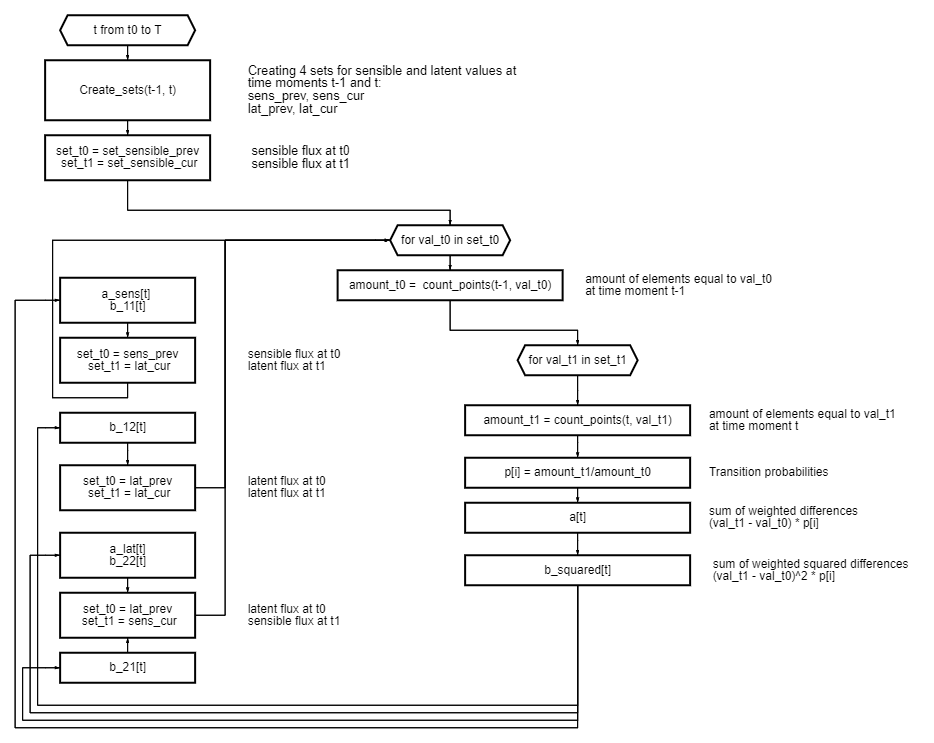
\includegraphics[width=\textwidth]{diagram_eng}
	\caption{Блок-схема алгоритма расчета оценок для коэффициентов $a$ и $b$} \label{fig:algo_nonparametric}
\end{figure}


Оценим вычислительную сложность этого алгоритма. Поскольку на каждом шаге $t \in [t_0,T]$ рассматриваются два момента времени $t_1$ и $t_2$, в которых присутствует вложенный цикл по уникальным значениям двух двумерных массивов, являющихся рассматриваемой сеткой, то сложность алгоритма будет составлять $O(t\times n^2)$, где $n$ – число элементов каждого из массивов. C учетом размеров рассматриваемой сетки, в текущей работе значения этих параметров следующие: $n=161\times181=29141$, $t = [0, 15917]$ - количество дней за рассматриваемый промежуток времени.


Расчет оценок коэффициентов $a$ и $b$, их корреляции и отношение $F$ выполнялись на высокопроизводительном кластере в индивидуальной вычислительной среде на основе технологии виртуальной контейнеризации docker. После выполнения всех расчетов для рассматриваемых величин были на локальной машине отрисованы графики в формате карт с последующей сборкой в видеофайлы формата mp4 продолжительностью около часа каждое.  
Программная реализация была выполнена на языке Python 3.7 с использованием библиотек Matplotlib, NumPy, Pandas, SciPy, Skimage, Seaborn, Xarray (для чтения grib-файлов) и др.

Исходные данные измерений явного и скрытого потока представляли собой 2 файла формата grib из открытой базы ERA5 (https://www.ecmwf.int/en/forecasts/datasets/reanalysis-datasets/era5), каждый из которых содержал в себе ежедневные измерения с шагом в $6$ часов за период 01.01.1979 -- 31.07.2022 на сетке с шагом в $0.5$ градуса со значениями широты в пределах $[-90, 0]$ и долготы в интервале $[0, 80]$ градусов. Для расчета коэффициентов данные были перегруппированы в numpy-массивы по десятилетиям (1979-1989гг., 1989-1999гг., 1999-2009гг., 2009-2019гг., 2019-2022гг.) с уменьшением размерности сетки до 1 градуса. Затем для выполнения расчетов с шагом в $1$ день данные были усреднены по $4$ подряд идущих измерения, за каждый день. Для выполнения расчетов оценок коэффициентов $a$ и $b$ данные предварительно дополнительно подвергались дискретизации, как подробно описано в разделе~\ref{sec:Disctretization}. Благодаря свойствам марковости рассматриваемых процессов стало возможно реализовать параллельный расчет на нескольких процессах-нитях с последующей сборкой результатов и обработкой границ интервалов родительским процессом, где параллелизм выполнялся по координате времени. 

Программы были зарегистрированы TODO \cite{progbib1, progbib2}

\section{Полупараметрический метод}
\label{sec:AlgoSemiparametric}
TODO блок-схема полупараметрического

\subsection{Выделение компонент связности}
\label{sec:ComponentsAlgo}
\begin{algorithm}[!h]
	\caption{Динамическое определение числа локальных компонент}
	\label{AlgGreedy}
	\begin{algorithmic}[1]
		\Function{NumGreedy}{Params, $ I^{(n)}$, $J^{(n+1)}$}
		\State  $I_0\gets \emptyset$, $J_0\gets \emptyset$, Comps$\gets \emptyset$;\Comment{{\em Инициализация}}
		\Repeat \Comment{{\em Продолжающиеся или новые компоненты}}
		\State \LongComment{{\em Оптимизация выражения~\eqref{I} с учетом условия~\eqref{Dist}}}
		\State [I, J]$\gets$\Call{FindI}{Params, $J^{(n+1)}\setminus J_0$, $I^{(n)}\setminus I_0$};
		\If{I $\neq \emptyset$}\Comment{{\em Найдена предшествующая $J$ компонента}}	
		\State $I_0\gets I_0\cup I$, $J_0\gets J_0\cup J$;
		\Else\Comment{{\em Добавление новой компоненты}}
		\State $J_0\gets J_0\cup J$;
		\State Comps $\gets$ \Call{AddNewComp}{Params, J};
		\EndIf
		\Until{($J^{(n+1)}\setminus J_0 \neq \emptyset$)}
		\State \Return Comps;
		\EndFunction
	\end{algorithmic}
\end{algorithm}

Предполагается, что данный алгоритм применяется для компонент с положительными весами (нулевые значения соответствуют случаю уменьшению их числа на каком-либо шаге). Кроме того, для всех допустимых значений $i\neq j$ и $n$ должны существовать такие $\delta_a>0$ и $\delta_\sigma>0$, что выполнено хотя бы одно из условий $\left|a_i^{(n)}-a_j^{(n)}\right|>\delta_a$, $\left|\sigma_i^{(n)}-\sigma_j^{(n)}\right|>\delta_\sigma$. Если же они оба нарушены, то необходимо объединять эти компоненты в одну с соответствующей корректировкой (суммированием) весов. То есть предполагается, что все компоненты различны, -- это гарантирует корректность применения жадного алгоритма.

Алгоритм~\ref{AlgGreedy} используется в качестве важной составной части  метода формирования матрицы связности. Она представляет собой вспомогательную структуру, в которую на каждом шаге скользящего окна сохраняется актуальное состояние всех выделенных к текущему моменту компонент. Сначала ко всему ряду применяется метод EM-типа для определения числа компонент на каждом шаге (как было отмечено выше, оно не может убывать). Затем в двухмерном пространстве $(a, \boldsymbol \sigma)$ используется один из методов кластеризации с полученным жадным алгоритмом числом локальных компонент-кластеров. Веса не учитываются, так как вклад компоненты в смесь может изменяться, при этом параметры -- математическое ожидание и дисперсия -- варьируются не слишком сильно и тогда считается, что это та же самая компонента. Соответствующая процедура представлена в алгоритме~\ref{AlgConnect}.

\begin{algorithm}[!h]
	\caption{Определение компонент связности в СРС-методе}
	\label{AlgConnect}
	\begin{algorithmic}[1]
		\Function {MSMComponents}{Data, options}
		\State Params $\gets$\Call{EMs}{Data, options.EM}\Comment{{\em СРС-метод}}
		\State \LongComment{{\em Инициализация числом ненулевых компонент на первом шаге}}
		\State  Comps$^{(1)}$$\gets$Params.k$^{(1)}$;
		\For{(n = 1:{length}(Params)-1)}
		\State Comps$^{(n+1)}$ $\gets$ \Call{NumGreedy}{Params, $ I^{(n)}$, $J^{(n+1)}$};
		\EndFor
		\State \LongComment{{\em Метки для каждого набора параметров, кластеризация}}
		\State Labels $\gets$ \Call{Clust}{Params, {max}(Comps), options.ClustAlg};
		\State \LongComment{{\em Матрица связности для компонент СРС-метода}}
		\State HistMatrConnect$\gets$ \Call{Сonnectivity}{Params, Labels};	
		\State \Call{PlotComp}{HistMatrConnect};\Comment{{\em Визуализация результатов}}
		\State \Return HistMatrConnect;
		\EndFunction
	\end{algorithmic}
\end{algorithm}

Очевидно, что данная процедура может быть использована и в случае смесей многомерных распределений. При этом в формулу оптимизации~\eqref{I} должны быть добавлены все параметры соответствующего распределения (с соответствующей модификацией условия~\eqref{Dist}), а затем может быть проведена кластеризация в пространстве переменных новой размерности.

Программы были зарегистрированы TODO \cite{progbib3, progbib4, progbib5, progbib6}

\section{Разложение Карунена-Лоэва}
\label{sec:AlgoKarhunen}
На рисунке \ref{fig:KarhunenAlgo} представлена блок-схема алгоритма разложения коэффициента диффузии на собственные вектора, описанного в разделе \ref{sec:Karhunen}.
\begin{figure}
	\centering
	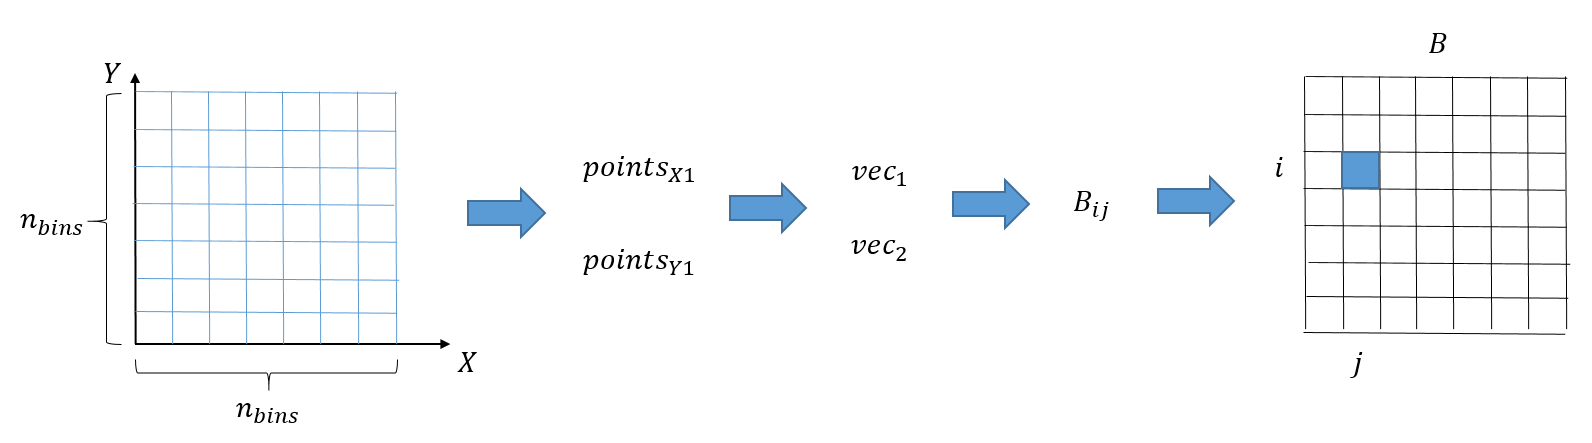
\includegraphics[width=\textwidth]{decomposition_concept.png}
	\caption{Блок-схема алгоритма разложения коэффициента диффузии}
	\label{fig:KarhunenAlgo}
\end{figure}



\section{Архитектура программного комплекса}
В этом разделе описана архитектура используемого программного комплекса.


\begin{figure}[!h]
	\centering
	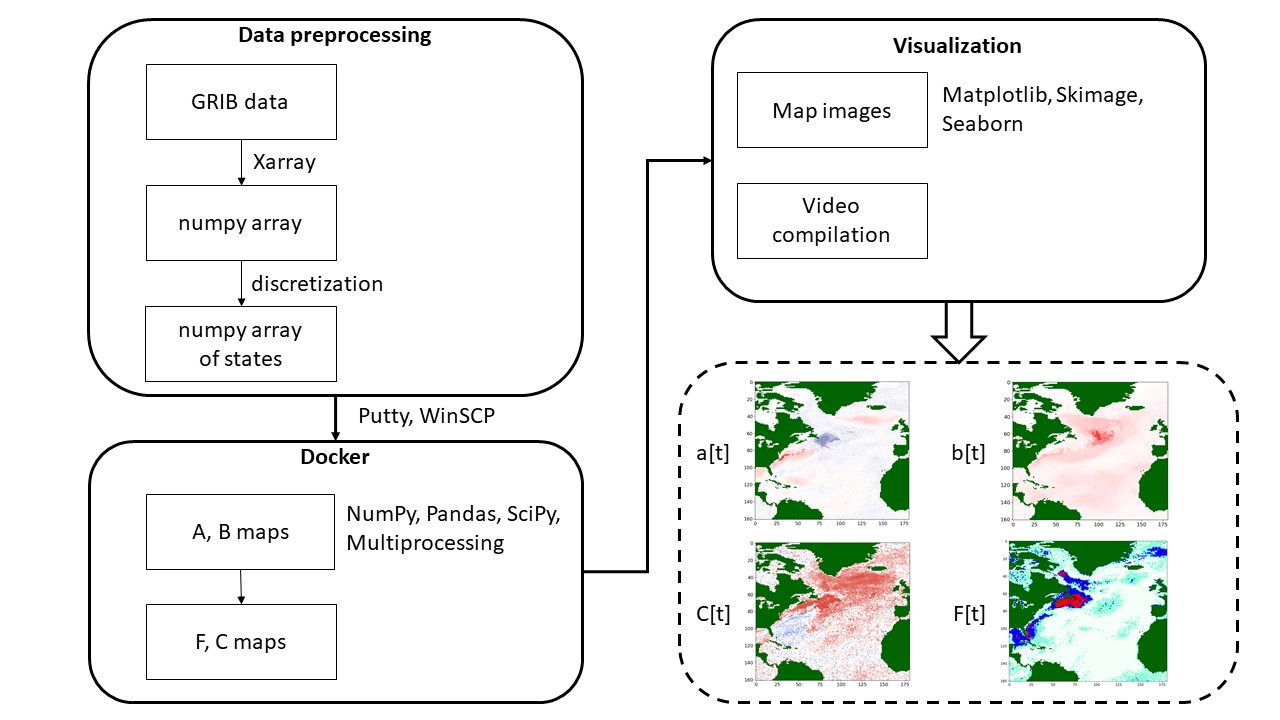
\includegraphics[width=0.99\textwidth]{scheme}
	\caption{Логическое представление архитектуры программного комплекса}\label{fig:app_scheme}
\end{figure}


На рисунке~\ref{fig:app_scheme} схематично показаны основные структурные компоненты проекта:
\begin{itemize}
	\item Блок \verb"Data prepocessing" содержит программные преобразование формата \verb"GRIB" (используется для хранения и передачи метеорологических данных с привязкой к сетке на двумерной географической карте) в тип данных \verb"NumPy", дискретизация (см. формулы~\eqref{eq:p_formula}--\eqref{eq:b_formula} и соответствующие пояснения к ним в разделе~\ref{sec:Nonparametic}).
	\item В блоке \verb"Docker" реализованы вычислительные алгоритмы (см. рисунок~\ref{fig:algo_nonparametric}) для расчет оценок коэффициентов $a$ и $b$, их корреляции и отношения $F$. Используется высокопроизводительный кластер архитектуры Intel x86\_64 (9 узлов на основе серверной платформы \verb"Huawei Server XH620": два \verb"Intel Xeon CPU E5-2683 v4" (2.1 GHz, 16 Core), 512 Gb RAM, 2*10G Ethernet, 2*16G \verb"FibreChannel") и индивидуальная облачная вычислительная среда на основе технологии виртуальной контейнеризации~\cite{peinl2016docker}.
	\item Блок \verb"Visualisation" предназначен для визуализации результатов: для рассматриваемых величин были на локальной машине отрисованы графики в формате карт с последующей сборкой в видеофайлы формата \verb"MP4" продолжительностью около часа каждое.
\end{itemize}

Для программной реализации использованы язык \verb"Python 3.7" и библиотеки \verb"Matplotlib", \verb"NumPy", \verb"Pandas", \verb"SciPy", \verb"Skimage", \verb"Seaborn", \verb"Xarray" (для чтения GRIB-файлов).

%На расчет оценок коэффициентов $a$ и $b$ ушло приблизительно $1.5$ дня непрерывных расчетов на кластере (включая накладные расходы), на расчеты $C$ и $F$ -- порядка двух часов. Отрисовка карт и сборка в видео-формат заняла около $3-4$ часов.




% \subsection{Physics-informed modification of the loss function}
% \label{section_informed_methodology}


% \new{The proposed physics-informed approach involves modifying the standard loss function, that is:
	% \begin{equation*}
		%     Loss(y_{true}, y_{predict})[i] = (1-\alpha) \cdot MSE(y_{true}, y_{predict})[i] + \alpha(t) \cdot (y_{predict} - A[i] - \sum_{j=1}^3 B_{ij} e_{ij})^2,
		% \end{equation*}
	% where $i\in \{1, 2, 3\}$ represents the variable index ($0$ for cumulative flux, $1$ for SST and $2$ for pressure),
	% \begin{equation*}
		% MSE=\frac1n\sum\limits_{j=1}n \left(y_{true}-y_{predict}\right)^2 
		% \end{equation*}
	% stands for standard mean squared error, $A_[i]$ are the estimates of the drift coefficient, $B_{ij}$ and $e_{ij}$,  $j \in \{1, 2, 3\}$ are the obtained estimations of the first eigenvalues and eigenvectors from the ordered set, and $\alpha(t)$ is the weight coefficient, that can be either a kind of hyperparameter or the self-adapting~\citep{Xiang2022} part of a neural network.
	% % , vanishing with each epoch number of the additional steps $t \in \{0, 1, \dots, 10\}$:
	% % $$
	% %     \alpha(t) = 0.6 \cdot 0.9^{-t}.
	% % $$
	% This modified loss function implements a variant of stochastic regularization to prevent the model from violating predictions, allowing neural networks to adjust to SDE limitations, and this can increase forecast quality.
	% }


